\subsection{Review:}\label{sc:review}

Looking back at the project the application sets out to do what it was designed to do, which was to create an application that uses augmented reality as a main game mechanic.
This main game mechanic can be seen in Figure \ref{fig:screent shot}.
Even though the final application is a success it doesn't mean there isn't room for improvement in the application and how it was developed.

\begin{figure}[ht!]
	\label{fig:screent shot}
	\centering
	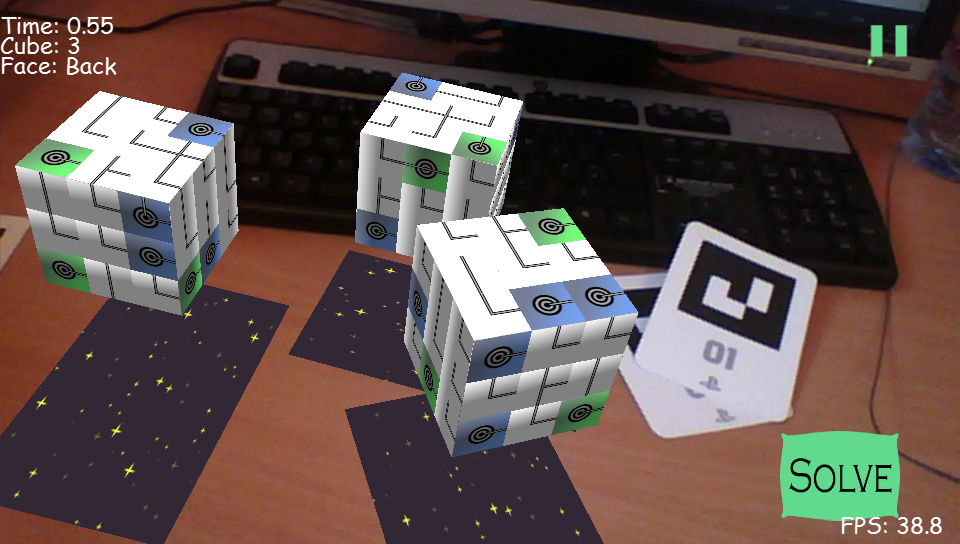
\includegraphics[width=\textwidth]{images/screenshot3.PNG}
	\caption{Application Screenshot}
\end{figure}

An example of this improvement is the use of encapsulation whilst developing the application.
Even though the application started with clear encapsulation between the objects and the main game class there are some areas, such as updating the selected face or cube, which are spread across multiple classes.
If the project were done again clearer encapsulation would be something that would be added.

Other improvements to the application can come in terms of the initial loading time.
The main culprit here is the loading of the puzzles from the text file.
If the loading time couldn't be improved it could be less noticeable if a loading or splash screen is added on start up.
Another small improvement can be via the completion of the menu system.
Even though the current application has working start and pause menus, the option menu haven't been finalised and could give access to extra feature such as audio.
Another feature that could be implemented could be a high score system that takes into account the time taken as well as the number of wrong solve checks selected.

The final improvement that could be made to the application would be to have different types of puzzles on the faces.
This would allow the user to play more variety of games which would curb any boredom that could occur from playing this type of game for a long period of time.
This could also help with the loading time issue depending on the types of puzzles or games on each face.